%%%%%%%%%%%%%%%%%%%%%%%%%%%%%%%%%%%%%%%%%%%%%%%%%%%%%%%%%%%%
%\subsection{Physics Objects}

\subsection{Leptons}
There are four tiers of lepton selections used in this analysis.
\begin{itemize}
  \item Inclusive selection for jet regression 
  \item Selection for jet cleaning
  \item Loose selection for Z boson reconstruction and additional lepton veto
  \item Tight selection for single lepton triggers and W boson reconstruction
\end{itemize}
\subsubsection{Electrons}
  Electrons are reconstructed with the Gaussian Sum Filter
  algorithm (GSF Electrons)~\cite{Khachatryan:2015hwa}. A tighter identification is then applied using a multivariate approach
  recommended by the electron-gamma (EGM) POG as documented here:

  \small{\texttt{https://twiki.cern.ch/twiki/bin/viewauth/CMS/ \\
  MultivariateElectronIdentificationRun2}}.
 
  A dedicated multivariate discriminator is trained for electrons that pass a set of cuts meant to reproduce
  the detector cuts applied by the most common electron triggers. 
  In this case, a set of offline cuts on ECAL-based electron quantities is applied
  on top of the multivariate discriminator to reproduce the conditions of the training sample:

  \texttt{pt>15 \& (}\\
  \texttt{(abs(superCluster().eta)<1.4442 \& full5x5\_sigmaIetaIeta<0.012 \& }\\
  \texttt{hcalOverEcal<0.09 \&}\\
  \texttt{(ecalPFClusterIso/pt)<0.4 \& (hcalPFClusterIso/pt)<0.25 \&}\\
  \texttt{(dr03TkSumPt/pt)<0.18 \& abs(deltaEtaSuperClusterTrackAtVtx)<0.0095 \&}\\
  \texttt{abs(deltaPhiSuperClusterTrackAtVtx)<0.065) || }\\
  \texttt{(abs(superCluster().eta)>1.5660 \& full5x5\_sigmaIetaIeta<0.033 \&}\\
  \texttt{hcalOverEcal<0.09 \&}\\
  \texttt{(ecalPFClusterIso/pt)<0.45 \& (hcalPFClusterIso/pt)<0.28 \&}\\
  \texttt{(dr03TkSumPt/pt)<0.18)}\\
  \texttt{).}

  Two cuts on the MVA ID discriminator~\cite{MVAeID} are applied
  defining two different working points based on the expected selection efficiency
  of either $90\%$ (loose, WP90) or $80\%$ (tight, WP80). The MVA working points are for the Spring 2016 training.
  
  \textbf{Inclusive selection for jet regression}: Electrons found inside jets are used to train the b-jet energy regression.
  We consider electrons for the quantities related to the leptons in jets,
  if they have $\pt > 5 \GeV$, $d_{xy}<0.5\cm$, $d_z<1.0\cm$, and no more than one expected missing
  inner tracker hits. 
  This selection is grandfathered in from the 76X Heppy framework for synchronization reasons,
  and should be reworked for the legacy analysis.
  More specifically, the GSF electron efficiency is known to drop substantially within heavy flavor jets
  due to the saturation of the ECAL, and most of the electrons selected this way are fakes.
  
  \textbf{Selection for jet cleaning}:
  Electrons are selected for jet cleaning by requiring $\pt>7\GeV$, $|\eta|<2.4$, $d_{xy}<0.05\cm$, $d_z<0.2\cm$ 
  (where both distances are taken with respect to the primary vertex), and a very loose relative
  isolation cut of 0.4, where the $\rho$-subtracted PF isolation in a cone of radius $0.3$ is used (Sec.~\ref{sec:leptiso}).
  The EGM scale corrections are currently applied to the electron $\pt$ before calculating this relative isolation.
  This is apparently not what was implemented in the 76X Heppy framework.

  \textbf{Loose selection}:
  Electrons which pass the Loose WP90 MVA working point are used to reconstruct Z bosons and for vetoing on additional leptons.
  The leading electron for Z boson reconstruction must have $\pt > 20\GeV$ for trigger threshold reasons.
  Otherwise, the electrons with $\pt > 15\GeV$ are used for the additional lepton veto.

  \textbf{Tight selection}:
  The tighter WP80 MVA working point is used in the \WenH\ channel to suppress the fake background in
  that final state. The tight electrons must also $\pt > 30\GeV$ and relative isolation $< 0.06$.
  To be clear, the same relative isolation and $\pt$ assignment are used as in the "Selection for jet cleaning."
  %in the \WenH\ and \ZeeH\ analyses, respectively, for the leading lepton. In the \ZeeH channel,
  %the trailing lepton is required to have $\pt$ in excess of $15\GeV$

\subsubsection{Muons}
  \textbf{Inclusive selection for jet regression:}:
  Muons found inside jets are also used to train the b-jet energy regression.
  We consider PF and global muons for the quantities related to the leptons in jets,
  if they have $\pt > 3 \GeV$, $d_{xy}<0.5\cm$, and $d_z<1.0\cm$.
  
  \textbf{Selection for jet cleaning}:
  The muons chosen for jet cleaning are PF muons reconstructed as either global or tracker muons, having $\pt>5\GeV$, $|\eta|<2.4$, $d_{xy}<0.5\cm$, $d_z<1.0\cm$, and
  relative isolation $< 0.4$, where the $\Delta\beta$-subtracted PF isolation in a cone of radius $0.4$ is used.

  \textbf{Loose selection}:
  The selection of muons for the Z boson reconstruction and the additional lepton veto is the same as
  the selection for jet cleaning, except that the leading (subleading) muon for Z boson
  reconstruction must have $\pt > 20 (10)\GeV$ for trigger threshold reasons.

  \textbf{Tight selection}:
  The tight muon selection is used in the \WmnH\ channel.
  It comprises muons having $\pt > 25\GeV$ and relative isolation $< 0.06$,
  which pass the following standard Tight ID cuts which have not changed since 2012:
 \begin{itemize}
  \item the candidate is reconstructed as a Global Muon:\\
  \texttt{isGlobalMuon()}
  \item Particle-Flow Muon:\\
  \texttt{isPFMuon()}
  \item $\chi^2/ndof$ of the global-muon track fit:\\
   \texttt{globalTrack()->normalizedChi2() < 10.}
  \item at least one muon-chamber hit included in the global-muon track fit:\\
  \texttt{globalTrack()->hitPattern().numberOfValidMuonHits() > 0 }
  \item muon segments in at least two muon stations; this implies that the muon is also an arbitrated tracker muon:\\
  \texttt{numberOfMatchedStations() > 1 }
  \item tracker track transverse impact parameter w.r.t. the primary vertex:\\
  \texttt{fabs(muonBestTrack()->dxy(vertex->position())) < 0.2 }
  \item longitudinal distance of the tracker track wrt. the primary vertex:\\
  \texttt{ fabs(muonBestTrack()->dz(vertex->position())) < 0.5 }
  \item number of pixel hits:\\
  \texttt{ innerTrack()->hitPattern().numberOfValidPixelHits() > 0 }
  \item cut on number of tracker layers with hits:\\
  \texttt{innerTrack()->hitPattern().trackerLayersWithMeasurement() > 5}
 \end{itemize}
  
\subsubsection{Lepton isolation\label{sec:leptiso}}

 Lepton isolation is defined starting from the PF isolation equation:
\begin{linenomath}\begin{equation}
  R\equiv \frac{\sum_i \left [ {\pt}_i(\texttt{chargedHadron}) + {\pt}_i(\texttt{neutralHadron}) + {\pt}_i(\texttt{Photon}) \right ]}{{\pt}^{\Pgm}}
\end{equation}\end{linenomath}

adding a term for subtraction of PU energy and momentum.  
This subtraction is based on the per-event estimated neutral energy expected to enter
a cone of radius $0.3$ ($0.4$) around the electron (muon) momentum. 
For electrons the estimate is obtained by computing the standard $\rho$ variable
using only neutral particle flow objects,
and then multiplying by a POG-estimated effective area of the cone (\texttt{Spring15\_25ns\_v1}).
For muons the correction is estimated from the deposit associated to charged tracks not belonging to the
primary vertex, with calibration factors given by the muon POG.   

Although the cuts are tight there is no loss in expected sensitivity and the data/MC agreement is very good in the bulk of the isolation distribution.

\subsection{Jets}

Jets used in the analysis are reconstructed by clustering particle flow candidates in the event using the anti-k$_{\rm T}$ algorithm \cite{Cacciari:2008gp} 
with a distance parameter of 0.4 and 0.8, constituting the AK4 and AK8 fatjets respectively. Details concerning their reconstruction follow.

The latest jet energy corrections are applied to data ({\tt Summer16\_23Sep2016[BCD,E,F,G,H]V3\_DATA}) and MC ({\tt Summer16\_23Sep2016V3\_MC}), following the JME POG recommendations~\cite{CMS-JEC-TWIKI}. 
Since the jet energy resolution (JER) differs in data and MC, in order to get a better agreement an additional smearing is applied to the simulation. The {\tt Spring1625ns\_V10} tag is currently used.

\subsubsection{AK4 Jets}
The official JME ``loose'' PF jet ID and the loose pileup ID are applied to the AK4 jets. We reject a jet if $\Delta {\rm R (jet,l)}<$~0.4 where $l$ is a preselected electron or muon.}

For the resolved categories, AK4 jets with $\pt > 25$ and $|\eta|<2.4$ are considered for building the \HBB system and for counting additional jets.
For the boosted AK8 fatjet categories, we define isolated jets, as AK4 jets with $\pt > 30$, $|\eta|<2.4$, and $\Delta {\rm R}>$~0.8 with respect to the highest
momentum AK8 fatjet. Applying b-tagging to the isolated jets allows us to reject or enhance the top-quark contribution in the signal and control regions.

\subsubsection{AK8 Fatjets}
To mitigate the effect of multiple interactions in the same bunch crossing, the pileup per particle identification (PUPPI) algorithm~\cite{Bertolini:2014bba} 
is used to weight the particle flow candidates prior to clustering the fatjets. This pileup jet discriminator is built based on event pileup properties, local shape and tracking information.
Further corrections are applied as a function of jet pseudorapidity($\eta$) and transverse momentum (L2,L3 corrections) to account for detector non-linearities.
Differences between data and simulation after L2 and L3 corrections are removed by applying a specific calibration to data events. Residual corrections are extracted from data using
the transverse momentum balance in $\gamma$+jets and Z+jets events~\cite{Chatrchyan:2011ds}. These corrections have been computed directly for AK8 PUPPI jets.

Subsequent to the clustering, we apply a jet grooming algorithm called "soft drop" which removes soft and wide-angle contributions from the jet, in order to mitigate the effects of contamination from initial state radiation (ISR), underlying event (UE) and pileup\cite{Larkoski:2014wba}.
Like any grooming method, soft drop declustering removes wide-angle soft radiation from a jet in order to mitigate the effects of contamination from initial state radiation (ISR), underlying event (UE), and multiple hadron scattering (pileup). Given a jet of radius $R_0$ with only two constituents, the soft drop procedure removes the softer constituent unless:

%\begin{linenomath}\begin{equation}
 $$\frac{\min(\pt^1,\pt^2)}{\pt^1+\pt^2} > z_{\mathrm{cut}} \left( \frac{\Delta R_{12}}{R_0} \right)^\beta$$
%\end{equation}\end{linenomath}
This algorithm controls the soft wide-angle radiation by a soft radiation fraction threshold $z_{\mathrm{cut}}$ and an angular exponent parameter $\beta$, where $\beta =0 $ corresponds roughly to the (modified) mass-drop procedure (mMDT) detailed in ~\cite{Dasgupta:2013ihk}. The default parameters used by CMS are $\beta=0$ and $z_{\mathrm{cut}}=1$.
The soft drop algorithm has the benefit of performing jet grooming in a theoretically safer way~\cite{Larkoski:2014wba,Larkoski:2013paa} and its behavior is constant across different clustering distance parameters~$R$ and \pt, which is not true for the pruning technique~\cite{Ellis:2009su,Ellis:2009me}.
Although the soft drop algorithm is primarly aimed at separating boosted \PW-jets from light quark/gluon-jets, it can fully reject contributions from underlying event and pileup when combined with the PUPPI algorithm.

The soft drop jet mass ($\mSD$) is the most important variable in the boosted fatjet categories. 
The $\mSD$ distribution peaks at the H mass for signal events, while the mass of background light quark- and gluon-initiated tends lower. 
The mass of top quark fatjets peaks at either the top quark mass, or the W boson mass if the top's b-quark daughter is not reconstructed inside the fatjet.

Specific corrections to the PUPPI soft drop mass are applied to correct for residual \pt-dependence, evaluated centrally by JMAR and documented in~\cite{AN-16-215}.
\begin{itemize}
  \item {\bf gen corrections}: a \pt-dependent correction to account for a small shift in the generated vector boson mass (derived for boosted W jet)
  \item {\bf reco corrections}: a \pt-dependent correction to the reconstructed jet mass, applied separately for jets in the barrel and endcaps regions
\end{itemize}

The shift in generated softdrop mass at lower \pt is of the order of 2-3\% while the difference between reconstructed and generated softdrop mass is a 5-10\% effect.
The mass shift introduced at generator level is corrected by a fit to $M_\textrm{PDG}/M_\textrm{GEN}$
as a function of jet \pt, where $M_\textrm{PDG} = 80.4$~\GeV and $M_\textrm{GEN}$ is the fitted mean of the generator level mass.
To correct for the residual shift between generator and reconstruction level, a fit to $(M_\textrm{RECO} − M_\textrm{GEN})/M_\textrm{RECO}$,
where $M_\textrm{RECO}$ is the reconstructed jet mass.

\subsubsection{Jet substructure}
\label{sec:substructure}

Jet substructure observables are used to distinguish boosted \PH bosons that decay hadronically from the hadronization products of single light quarks or gluons,
as well as top quarks.
Examples of observables widely used in jet substructure include $N-$~subjettiness ratios~\cite{Thaler:2010tr} and energy correlation functions (ECFs)~\cite{Larkoski:2013eya}.
These are usually constructed using power counting techniques, from a basis of infrared and collinear (IRC)\footnote{A general
IRC safe observable, insensitive to the emission of soft or collinear gluons, can be constructed using all energy deposits and angular information of a hard scattering event.}
safe observables that probe $N-$prong substructure within a jet.
Power counting~\cite{Larkoski:2014gra} can predict which combinations of observables are optimally sensitive to specific parametric features within a jet and can elucidate the underlying physics probed by the observables.

The quantity \textbf{N-subjettiness}~\cite{Thaler:2010tr,Thaler:2011gf,Stewart:2010tn} $\tau_N$ is used to quantify the degree to which jet constituents can be arranged into N subjets. It is defined as:

\begin{equation}
\tau_{N} = \sum_{1 \leq i \leq n_{J}}{z_{i} \min\{\Delta R_{i1}^{\beta},...,\Delta R_{iN}^{\beta}\}},
\end{equation}

where $z_{i}$ refers again to the energy fraction, and $\Delta R_{iK}$ refers to the angular separation between the constituent $i$ and the subjet axis $K$ in the jet. In particular, the ratio of ``$2-$~subjettiness'' to ``$1-$~subjettiness'' ($\tau_{2}/\tau_{1}$ = $\tau_{21}$) is designed to take small values for a jet with well-resolved 2-prong substructure, and has therefore, excellent capability at separating jets originating from boosted vector bosons from jets originating from quarks and gluons. The ratios $\tau_2/\tau_1$ and $\tau_3/\tau_2$ are calculated for the $\PH(\bbbar)$ fatjet, where the latter is aimed at reducing the amount of top quark background.

$N-$~subjettiness~($\tau_{N}$) divides a jet into $N$ sectors and correlates the particles in each sector with their corresponding axis. 
Thus, the definition of N-subjettiness requires an implicit definition of appropriate N-subjettiness axes, which can lead to different behaviors of the observable. In this context,
a new basis of IRC safe observables was recently proposed in~\cite{Moult:2016cvt}. These observables, named as generalized energy correlation functions ($_{o}e_{n}^{\beta}$), are defined as follows:

\begin{equation}
_{o}e_{n}^{\beta} = \sum_{1\leq i_{1}<i_{2}<...<i_{n}\leq n_{J}}{\prod_{1\leq k \leq n}{z_{i_{k}}}} \times \color{black}{\min \{ \prod_{s<t\in \textrm{pairs}\{i_1,i_2,...,i_n\}}^{o} {\Delta R_{st}^{\beta}}\} }\color{black},
\label{eq:ecfs}
\end{equation}

where:

\begin{itemize}
\item $n$, denotes the number of particles to be correlated i.e. the order of the correlation function. For an $n-$~pronged jet, $e_{n} >> e_{m}$, for $m \geq n$.
\item $o$, denotes the order of the angular factor, and
\item $\beta$, is related to the angular weighting.
\end{itemize}

The $_{o}e_{n}^{\beta}$ correlate $o$ pairwise angles among $n$ particles, allowing high flexibility in angular scaling. Furthermore, we define dimensionless ratios of the energy correlation functions as:

\begin{equation}
\psi(a,\alpha,N;b,\beta,M) = \frac{e(a,N,\alpha)}{e(b,M,\beta)^x}\text{, where } M\leq N\text{ and }x=\frac{a\alpha}{b\beta}
\label{eq:psi}
\end{equation}

In the boosted fatjet category of the \WenH\ and \WmnH\ channels, we use several dimensionless ratios of the 4-point and 3-point correlations to separate the \HBB\ signal from 
top quark background in the event classifier BDT.

\subsection{Missing Transverse Energy}

The $\MET$ used in the analysis is computed by taking the negative vector sum of the transverse momenta of all particle flow candidates reconstructed in a given event. Corrections to the momenta of jets reconstructed in the event are further propagated to the $\MET$ (Type-1 corrections).%, weighted with weights calculated by the PUPPI algorithm. Corrections to the momenta of jets reconstructed in the event are further propagated to the $\MET$ (Type-1 corrections).
Events in data can end up with large spurious $\MET$ due do detector noise and beam backgrounds.
In order to remove these events several $\MET$ filters have been recommended by the JetMET POG and have been implemented in the analysis.

\begin{center}

\href{https://twiki.cern.ch/twiki/bin/view/CMS/MissingETOptionalFiltersRun2}{\texttt{https://twiki.cern.ch/twiki/bin/view/CMS/MissingETOptionalFiltersRun2}}

\end{center}


In the \WenH\ and \WmnH\ channels, the $\MET$ is used along with the tight lepton that passes the trigger to build the W boson momentum in the transverse plane.

The significance of the missing transverse energy (METsig) assesses, on an event by event basis, the likelihood that an observed MET is consistent with a fluctuation from zero because of detector-related limitations like finite measurement resolution. The variable is used to reject QCD-like events with no genuine MET:

\begin{center}

\href{https://twiki.cern.ch/twiki/bin/view/CMSPublic/SWGuideMETSignificance}{\texttt{https://twiki.cern.ch/twiki/bin/view/CMSPublic/SWGuideMETSignificance}}

\end{center}

\subsection{B-tagging\label{sec:bjets}}
\subsubsection{CMVA for AK4 jets}
The identification of AK4 jets that originate from the hadronization of $\PQb$ quarks
is done with the Combined MVA v2 (cMVAv2)     algorithm~\cite{Chatrchyan:2012jua} with \texttt{PAT} string:
\begin{center}
\texttt{pfCombinedMVAV2BJetTags}
\end{center}
(while for the previous iteration of the analyses we have instead used the Combined Secondary Vertex CSVv2 algorithm).
The CMVAv2 algorithm provides a continuous discriminator output combining
in an optimal way the information about track impact parameters and identified secondary 
vertices within jets,  even when full vertex information is not available, and information of any soft lepton present in the jet.  Additional
categories for jets where a ``pseudo vertex'' is found, or no vertex at all is identified,
can be defined and combined in a multivariate discriminant (Boosted Decision Tree) to provide maximal separation
of b jets from the much larger background of jets arising from charm decay, and from the
fragmentation of light quarks and gluons.

The CMVAv2 output that can be used to select 
optimal working points with respect to the VH analyses, in addition to the standard 
Loose/Medium/Tight working points defined by the BTV POG: CMVAv2L $(>-0.5884)$, 
CMVAv2M $(>0.4432)$, and CMVAv2T $(>0.9432)$.
Independent optimizations of the selection criteria in all five channels arrive at roughly the same 
optimal selection for the jet in the Higgs decay that has the higher value of the CMVAv2
output: very close to the CMVAv2T working point. For the second jet, the optimal selection 
typically falls between the CMVAv2L and CMVAv2M working points.

The calibration of the CMVAv2 discriminator is determined using a tag-and-probe method
as documented in Ref.~\cite{bTagWeight}.
This method attempts at correcting the distribution of the CMVAv2 discriminator for simulated jets
as to match the distribution observed in data control regions.
These control regions are preselected by the requiring at least two opposite-sign leptons
plus at least two jets. Two exclusive set of selections based on the dilepton mass and the CMVAv2 discriminator or
a ``tag'' jet are further imposed to enrich the control regions in Z+jets or $\mathrm{t\bar{t}}$, respectively.
The binned CMVAv2 distribution of the ``probe'' jet is the compared to the one expected from simulation. An iterative
procedure is then initiated to scale every bin content in the simulation simultaneously for light and heavy flavour jets
(\texttt{hadronFlavour()=0} and \texttt{hadronFlavour()=5}, respectively). This procedure is carried out for various
$\pt$ and $|\eta|$ bins 
The ratio between the re-scaled distribution in the simulated sample and the original one is used as a jet-by-jet 
weight, $w_j$, defined as
\begin{linenomath}\begin{equation}
w_j(\mathrm{CMVAv2}_j;{\pt}_j,|\eta_j|,\mathrm{flavour}_j).
\end{equation}\end{linenomath}
By construction, the weights average to one when sampling CMVAv2 using the distribution predicted by the
simulation: $N^{-1}\sum_{i=1}^{N} w_j \to 1$, for $N>>1$ jets. 
In an event with $N_{\mathrm{jet}}$ selected jets whose CMVAv2 discriminator is used in the analysis,     
an event weight $w$ is defined starting from the jet weights as:
\begin{linenomath}\begin{equation}
w = \prod_{j=1}^{N_{\mathrm{jet}}} w_j(\mathrm{CMVAv2}_j;{\pt}_j,|\eta_j|,\mathrm{flavour}_j).
\end{equation}\end{linenomath}

\subsubsection{Double b-tag for AK8 fatjets}
In order to identify candidate Higgs fatjets containing two b quarks,
we use the double \cPqb-tagger discriminant~\cite{CMS-PAS-BTV-15-002}.

A brief description of the double-b tagger algorithm is as follows:
Tracks and secondary vertices associated to a jet are used, as for standard \cPqb-tagging.
The tracks are used to calculate the axes of N-subjettiness in the fatjet, by defining an axis for each prong which are used as input to the double-b tagger, instead of the jet-direction.
The two $\tau$-axis directions are used to resolve the two B-hadron decay chains we expect for a X to \bbbar\ signal.
Secondary vertex observables are assigned to each axis independently of the subjet components.
Then, b-tagging observables are computed using displaced tracks, secondary vertices (SV), and two-SV system information.
This dedicated tagger represents an alternative for boosted topologies to the subjet b-tag which relies on the subjet definition which breaks down at higher \pt.

For this analysis, we cut on the medium working point of 0.8 to gather events with real boosted \bbbar\ pairs.
The efficiency for passing this cut differs between data and simulation.
This is accounted for by applying a Data/MC scale factor to the efficiency.
The signal scale factor is measured centrally by the BTV POG, and is applied to the efficiency for the true VH(bb) signal,
as well as the highly signal-like \ensuremath{\mathrm{V+\bbbar}}\ backgrounds.
The mistag efficiency scale factors for the \ttbar\ and V+light flavor jets backgrounds are each measured in situ, by
adding to the maximum likelihood fit a Gaussian-constrained nuisance parameter for the simulated efficiency
which is adjusted for the Data/MC discrepancy by an unconstrained nuisance parameter.

The mistag scale factor for \ttbar\ is also measured centrally by the BTV POG, providing a useful cross-check that our
model is correct and unbiased. We measure the \ttbar mistag scale factor to be $\mathbf{1.09 \pm 0.02}$, which is
to be compared with the central numbers $\mathbf{1.05 \pm 0.04}$ (for $\pt < 350 \GeV$) and $\mathbf{1.09 \pm 0.08}$ (for $\pt < 700 \GeV$).
No such cross-check exists for the V+LF mistag scale factor, which is one of the dominant uncertainties in the boosted category.
One way to improve the boosted category sensitivity, if time permits, would be to measure it independently
to provide an initial constraint.

Because the shape of the double b-tag is mismodeled, and corrections for this are not available,
we cannot use the actual discriminator value as an input for the signal extraction BDT.
Future plans including upgrading to a deep neural network implementation for double b-tagging, which was recently integrated centrally in CMSSW.
This can benefit from the same in situ scale factor strategy if the central numbers become available in time.

\subsection{Soft activity calculation}\label{sec:soft}
For the VH signal events, not much additional hadronic activity is expected
after excluding the V and H decay products.
The additional soft activity is defined as follows.
We make only use of charged tracks that clearly originate from the event main interaction point
to monitor the additional radiation.
As described above, the main interaction point in the event is defined as the ``hardest''
reconstructed primary vertex (PV),
i.e. with the largest \pt$^2$ sum for the tracks that have been used to reconstruct it.

At first a collection of soft additional tracks is built using reconstructed tracks that 
\begin{itemize}
\item  have a  {\em high purity} quality flag ,
\item have $\PT>300~\MeVc$,
\item are not associated to the vector decay leptons, nor to the selected two b-jets in the event 
(through the PF candidates components track references),
\item make minimum $|d_z({\rm PV})|$ when associated to the event hardest primary vertex (PV), 
\item satisfy $|d_z({\rm PV})|<$~2~mm with respect to the hardest PV.
\end{itemize}

In addition to removing the tracks in the jets, also tracks in 
the region between the two b-jets are removed by defining a ellipse in 
the $\eta\phi$ plane around the two b-jets with axes $(a,b)= (\Delta R({\rm bb})+1,1)$,
and excluding all tracks pointing within the ellipse from the additional tracks collection.
A schematic of this is shown in Figure~\ref{fig:softActivity}.

\begin{figure}[tbp]
  \begin{center}
    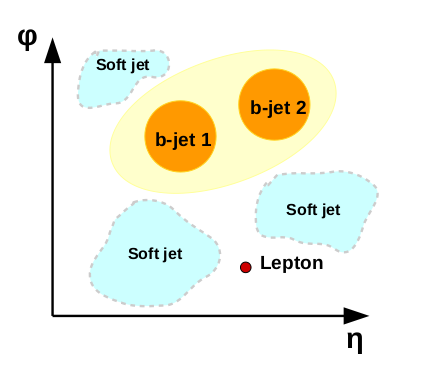
\includegraphics[width=0.48\textwidth]{figures/wlnhbb2016/softActivitySchematic.png}
    \caption{Schematic diagram for the exclusion of tracks for the soft activity calculation.}
    \label{fig:softActivity}
  \end{center}
\end{figure}

After this track selection, a collection of soft track jets is built clustering the aforementioned soft additional tracks
with the anti-$k_{\rm T}$ clustering algorithm~\cite{Cacciari:2008gp} with distance parameter $R=0.4$.
The use of track-jets represents a clean and commissioned method~\cite{CMS-PAS-JME-10-006} to reconstruct
the hadronization of partons with very low energies, down to few GeV~\cite{CMS-PAS-JME-08-001}.

For the purpose of separating the signal from backgrounds, we consider:
\begin{itemize}
\item the scalar $\pt$ sum of the soft track jets with transverse momentum $\pt>1~\GeV$, $H_T^{\rm soft}$; 
\item the soft track jet multiplicity $N^{\rm soft}$ with transverse momentum $\pt>2~\GeV$, $N_2^{\rm soft}$;
\item the soft track jet multiplicity $N^{\rm soft}$ with transverse momentum $\pt>5~\GeV$, $N_5^{\rm soft}$;
\item the soft track jet multiplicity $N^{\rm soft}$ with transverse momentum $\pt>10~\GeV$, $N_{10}^{\rm soft}$;
\end{itemize}

The soft activity is used as a discriminating variable in the signal extraction BDT for the resolved categories.


\subsection{Top(bW) mass reconstruction}\label{sec:topmass}

In the resolved \WlnHbb\ categories,the background from \ttbar\ production is problematic
and grows faster with $\sqrt{s}$ than Higgs boson production.
Therefore, several variables were analyzed to help further discriminate against 
this background. In the end, the reconstructed top mass was included as an 
analysis variable because of its discrimination power.

\WlnHbb\ events are characterized by the presence of an isolated lepton, 
$\MET$, and two b-jets.  This is the same signature for semi-leptonic \ttbar\ 
events.  Furthermore, the lepton and the $\MET$ should both arise from the 
decay of the W boson.  Assuming this W boson is exactly on shell as a constraint,
we solve an equation with lepton \pt\, W mass, known \pt\ of the neutrino 
(assumed to be equal to $\MET$) and unknown longitudinal neutrino momentum.

\begin{eqnarray}
M_{W}^2 & = & (E_{\nu}+E_{\ell})^2-(\overrightarrow{p_{\nu}}+\overrightarrow{p_{\ell}})^2
\end{eqnarray}

There are always two solutions to this equation.  When both are real, the 
solution with the smaller longitudinal neutrino momentum is selected.  When 
the solutions are imaginary, the real part is taken as the longitudinal 
neutrino momentum.

Once this is done, the 4-momenta of the neutrino, the lepton,
and the closest b-jet are added to furnish the top quark's invariant mass.
